\documentclass{standalone}
\usepackage{tikz}
\usetikzlibrary{fit}
\usetikzlibrary{calc}

\begin{document}
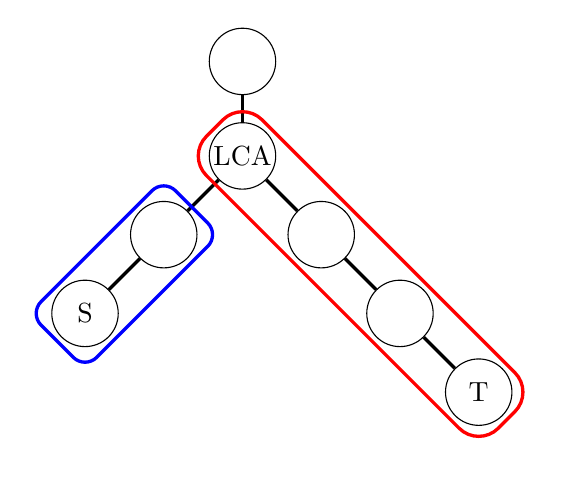
\begin{tikzpicture}[every node/.style={circle,draw,minimum size=24pt,inner sep=0pt}]

% 节点
\node (s) at (0,0) {S};
\node (a) at (1,1) {~};      % use ~ for empty nodes
\node (lca) at (2,2) {LCA};
\node (x) at (2,3.2) {~};
\node (b) at (3,1) {~};
\node (c) at (4,0) {~};
\node (t) at (5,-1) {T};

% 边
\draw[very thick] (s) -- (a) -- (lca) -- (b) -- (c) -- (t);
\draw[very thick] (lca) -- (x);

% 蓝色倾斜矩形框(S到LCA的左儿子)
\draw[blue,very thick,rounded corners=6pt,rotate around={-45:(a)}]
  ($(s)+(-0.5,-0.5)$) rectangle ($(a)+(0.5,0.5)$);

% 红色倾斜矩形框(LCA到T)
\draw[red,very thick,rounded corners=10pt,rotate around={45:(c)}]
  ($(lca)+(-0.5,0.5)$) rectangle ($(t)+(0.5,-0.5)$);

\end{tikzpicture}
\end{document}